\chapter{SP2-CU14 Agregar comentarios a propuesta de unidad de aprendizaje}
\begin{UseCase}{SP2-CU14}{ Agregar comentarios a propuesta de unidad de aprendizaje }{El usuario podrá agregar uno o más comentarios en la sección de propuesta de unidad de aprendizaje que está revisando.}
		\UCitem{Versión}{\color{Gray}1.0}
		\UCitem{Autor}{\color{Gray}Romero Ponce Mauricio Isaac}
		\UCitem{Supervisa}{\color{Gray}Parra Garcilazo Cinthya Dolores}
		\UCitem{Actor}{Analista}
		\UCitem{Propósito}{Asignar cuales son y donde están las correcciones que se deben realizar a la sección de la unidad de aprendizaje que se está revisando.}
		\UCitem{Entradas}{Las dos entradas para agregar un comentario en una sección de la propuesta de unidad de aprendizaje son:
          \begin{itemize}
          	\item Posición en la que se agregará el comentario.
          	\item Comentario.
           % \item fecha en que se genera el nuevo comentario.
            %\item Identificador unico del analista.
          \end{itemize}
        }
		\UCitem{Origen}{Mouse y teclado.}
		\UCitem{Salidas}{
        	\begin{itemize}
        		\item MSG1. La operación se ha realizado con éxito.

                \item MSG2. Error: Primero se debe seleccionar el punto en donde se agregará el comentario.
                \item MSG3 Error: debe agregar un texto al nuevo comentario.
                \item MSG4 Ingrese su comentario en el nuevo campo de la bitácora.
        	\end{itemize}
        }
		\UCitem{Destino}{Pantalla.}
		\UCitem{Precondiciones}{ Se llamó el caso de uso SP2-CU7 o SP2-CU8 o SP2-CU9 o SP2-CU10 o  SP2-CU11 o o SP2-CU12}
		\UCitem{Postcondiciones}{
            \begin{itemize}
                \item Se agregará al sistema el comentario.
                \item Se mostrará en la bitácora el comentario
                \item Se habilita la llamada a los casos de uso SP2-CU15 y SP2-CU16  
             \end{itemize}  
        }
		\UCitem{Errores}{}
		\UCitem{Estado}{Revisión.}
		\UCitem{Observaciones}{}
\end{UseCase}

%--------------------------- CU TRAYECTORIA PRINCIPAL -------------------------
\begin{UCtrayectoria}{Principal}

    \UCpaso[\UCactor] Selecciona con el mouse el texto donde pondrá un comentario.

    \UCpaso[\UCactor] Presiona el botón \IUbutton{Nuevo comentario}. \hyperref[SP2-CU14-A]{Trayectoria A}. 
    
    \UCpaso Obtiene la fecha de la fecha actual. 
    
    \UCpaso Obtiene la clave del usuario que desea agregar un comentario.
    
    \UCpaso Muestra el nuevo comentario en el costado derecho del documento a la altura en que se seleccionó el texto del paso 1. \hyperref[SP2-CU14-B]{Trayectoria B}.
    
    \UCpaso Muestra el mensaje \MSGref{MSG4}.

    \UCpaso[\UCactor] Cierra el mensaje presionando \IUbutton{Aceptar}.
    
    \UCpaso[\UCactor] Ingresa el nuevo comentario en el input text "comentario".
    
    \UCpaso[\UCactor] Presiona el botón \IUbutton{Aceptar}. \hyperref[SP2-CU14-C]{Trayectoria C}.
    
    \UCpaso Verifica que el campo comentario haya sido contestado. \hyperref[SP2-CU14-D]{Trayectoria D}.

    \UCpaso Guarda la información del nuevo comentario en la base de datos.

    \UCpaso El sistema muestra el  \MSGref{MSG1}.

    \UCpaso[\UCactor] Cierra el mensaje presionando \IUbutton{Aceptar}.

    \UCpaso desaparecen los botones  \IUbutton{Aceptar} y  \IUbutton{Cancelar}.

    \UCpaso Aparecen los botones  \IUbutton{Editar} y  \IUbutton{Eliminar}.

\end{UCtrayectoria}

%------------------------ CU TRAYECTORIA ALTERNARIVA A -------------------------
\label{SP2-CU14-A}
\begin{UCtrayectoriaA}{A}{El usuario no seleccionó alguna parte del texto.}

	\UCpaso El sistema detecta que no hay referencia en el texto para el nuevo comentario.

  \UCpaso El sistema muestra el \MSGref{MSG2}.

  \UCpaso[\UCactor] Cierra el mensaje presionando \IUbutton{Aceptar}.

  \UCpaso continúa en el paso 1 de la trayectoria principal del CU-V14.
\end{UCtrayectoriaA}

%------------------------ CU TRAYECTORIA ALTERNARIVA B -------------------------
\label{SP2-CU14-B}
\begin{UCtrayectoriaA}{B}{El sistema detecta un comentario ya existente en el mismo renglón que el nuevo comentario.}

    \UCpaso Genera el comentario nuevo debajo del comentario ya existente. 
    \UCpaso continúa en el paso 6 de la trayectoria principal del CU-V14.
\end{UCtrayectoriaA}

%------------------------ CU TRAYECTORIA ALTERNARIVA C -----------------------
\label{SP2-CU14-C}
\begin{UCtrayectoriaA}{C}{El usuario presionó \IUbutton{Cancelar}}

	\UCpaso Elimina el comentario generado previamente.
\end{UCtrayectoriaA}

%------------------------ CU TRAYECTORIA ALTERNARIVA D -----------------------
\label{SP2-CU14-D}
\begin{UCtrayectoriaA}{D}{El sistema detecta que el campo “comentario” se encuentra vacío.} 

	\UCpaso Muestra el \MSGref{MSG3}.
    \UCpasoEl sistema muestra el mensaje \MSGref{MSG4}.

    \UCpaso[\UCactor] Cierra el mensaje presionando \IUbutton{Aceptar}.

    \UCpaso Continúa en el paso 8 de la trayectoria principal del CU-V14.
\end{UCtrayectoriaA}

\chapter{Pantallas}
 \begin{figure}
  \centering
    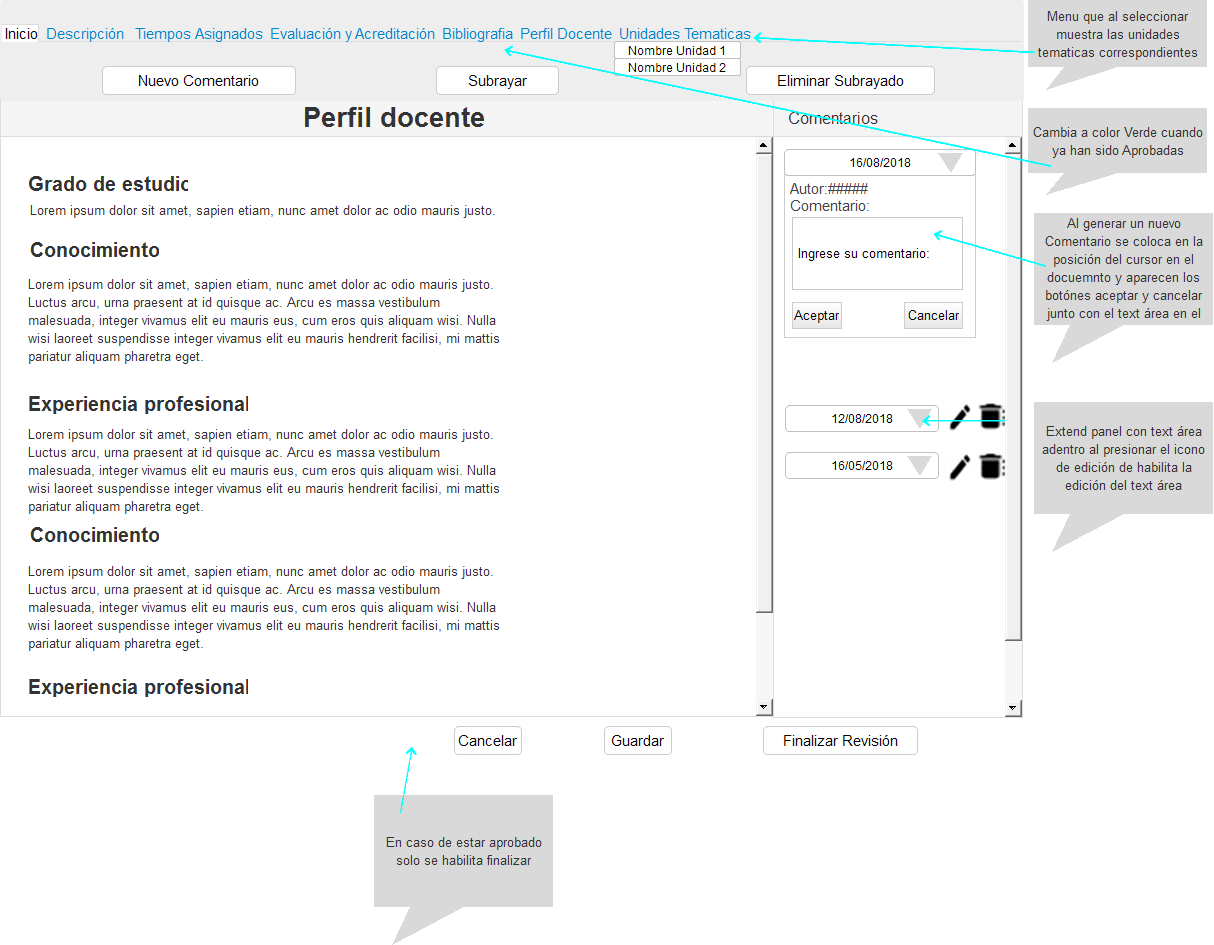
\includegraphics[width=0.7\textwidth]{DCU/SP2/Pantallas/Nuevo_comentario}
  \caption{SP2-IU-Nuevo comentario}
  \label{SP2-IU-Nuevo_comentario}
\end{figure}
